% Source: graduate-coursework/Sp26/CSCE775/HW1/HW1_CSCE_775_solutions.tex

\documentclass[border=4pt]{standalone}
\usepackage{amsmath}
\usepackage{amssymb}
\usepackage{bm}
\usepackage{graphicx}
\usepackage{pgfplots}
\usepackage{tikz}
\usepackage{xcolor}
\pgfplotsset{compat=1.18}
\usetikzlibrary{shapes.geometric, arrows.meta, positioning, automata, calc, decorations.markings, patterns}

\definecolor{USC_Garnet}{HTML}{73000A}
\definecolor{USC_Sandstorm}{HTML}{FFF2E3}
\definecolor{USC_Black90}{HTML}{363636}
\definecolor{USC_Black70}{HTML}{5C5C5C}
\definecolor{USC_Black50}{HTML}{A2A2A2}
\definecolor{USC_Black10}{HTML}{ECECEC}
\definecolor{USC_Honeycomb}{HTML}{A49137}
\definecolor{USC_Horseshoe}{HTML}{65780B}
\definecolor{USC_Atlantic}{HTML}{466A9F}
\definecolor{USC_Congaree}{HTML}{1F414D}
\definecolor{USC_Rose}{HTML}{CC2E40}


\begin{document}
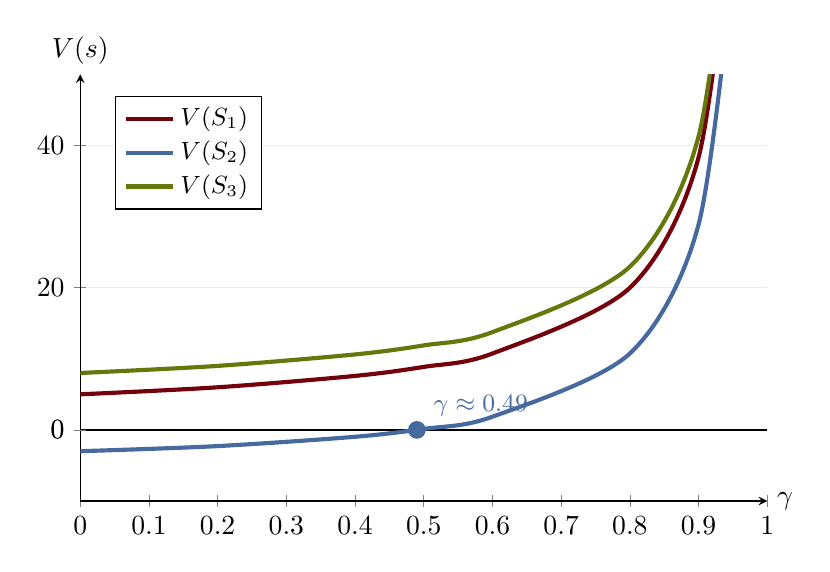
\begin{tikzpicture}
\begin{axis}[
    width=0.85\textwidth,
    height=7cm,
    xlabel={$\gamma$},
    ylabel={$V(s)$},
    xmin=0, xmax=1,
    ymin=-10, ymax=50,
    ymajorgrids=true,
    grid style={USC_Black10},
    axis lines=left,
    every axis x label/.style={at={(ticklabel* cs:1.0)}, anchor=west},
    every axis y label/.style={at={(ticklabel* cs:1.0)}, anchor=south},
    extra y ticks={0},
    extra y tick style={grid=major, grid style={black, line width=0.5pt}},
    legend style={at={(0.05,0.95)}, anchor=north west, font=\small},
]
% V(S1)
\addplot[color=USC_Garnet, line width=1.5pt, mark=none, smooth]
    coordinates {
        (0, 5.00) (0.2, 5.99) (0.4, 7.59) (0.5, 8.86)
        (0.6, 10.74) (0.8, 19.99) (0.9, 38.33) (0.95, 74.91)
    };
\addlegendentry{$V(S_1)$}

% V(S2)
\addplot[color=USC_Atlantic, line width=1.5pt, mark=none, smooth]
    coordinates {
        (0, -3.00) (0.2, -2.28) (0.4, -0.97) (0.5, 0.14)
        (0.6, 1.85) (0.8, 10.75) (0.9, 28.89) (0.95, 65.37)
    };
\addlegendentry{$V(S_2)$}

% V(S3)
\addplot[color=USC_Horseshoe, line width=1.5pt, mark=none, smooth]
    coordinates {
        (0, 8.00) (0.2, 9.00) (0.4, 10.61) (0.5, 11.88)
        (0.6, 13.75) (0.8, 22.96) (0.9, 41.27) (0.95, 77.83)
    };
\addlegendentry{$V(S_3)$}

% Zero-crossing marker
\addplot[only marks, mark=*, mark size=3pt, color=USC_Atlantic]
    coordinates {(0.49, 0)};
\node[anchor=south west, font=\small\bfseries, text=USC_Atlantic] at (axis cs:0.50, 0.5) {$\gamma \approx 0.49$};

\end{axis}
\end{tikzpicture}
\end{document}
